\documentclass{article}

\usepackage{ewrl_2026}

\usepackage[utf8]{inputenc}
\usepackage[T1]{fontenc}
\usepackage{hyperref}
\usepackage{url}
\usepackage{booktabs}
\usepackage{amsfonts}
\usepackage{amsmath, amssymb}
\usepackage{nicefrac}
\usepackage{microtype}
\usepackage{xcolor}
\usepackage{graphicx}
\usepackage{subcaption}
\usepackage{algorithm}
\usepackage{algpseudocode}
\usepackage{tikz}
\usetikzlibrary{arrows.meta, positioning, shapes.geometric, fit, backgrounds}

\newcommand{\physigym}{\textsc{PhysiGym}}
\newcommand{\physicell}{\textsc{PhysiCell}}
\newcommand{\Itwo}{\texttt{img\_mc\_cells\_substrates}}
\newcommand{\Ione}{\texttt{img\_mc\_cells}}
\newcommand{\Sone}{\texttt{scalars\_cells}}
\newcommand{\Stwo}{\texttt{scalars\_cells\_substrates}}
\newcommand{\Sthree}{\texttt{spatial\_scalars\_cells}}
\newcommand{\Sfive}{\texttt{spatial\_scalars\_cells\_spatial\_substrates}}

% ─────────────────────────────────────────────────────────────────────────────

\title{\physigym{}: Bridging Agent-Based Biological Simulation and Reinforcement
  Learning  A State-Space Study on Tumor Microenvironment Control}

\author{%
  Alexandre Bertin$^{1,2,5,\dagger}$ \quad
  Elmar Bucher$^{3,\dagger}$ \quad
  Owen Griere$^{2,5}$ \quad
  Marcelo Hurtado$^{2,5}$ \\
  Heber Rocha$^{3}$ \quad
  Randy Heiland$^{3}$ \quad
  Paul Macklin$^{3,\ddagger}$ \quad
  Vincent Fran\c{c}ois-Lavet$^{4,\ddagger}$ \\
  Emmanuel Rachelson$^{1,\ddagger}$ \quad
  Vera Pancaldi$^{2,5,\ddagger}$ \\[4pt]
  $^1$CRCT, Univ Toulouse, INSERM, CNRS, CRCT, Toulouse, France \\
  $^2$ISAE-Supaéro, Toulouse, France \quad
  $^3$Dept.\ of Intelligent Systems Engineering, Indiana University, USA \\
  $^4$Dept.\ of Computer Science, VU Amsterdam, The Netherlands \quad
  $^5$Equipe Labélisée Ligue Nationale Contre le Cancer, France \\[2pt]
  {\small $^\dagger$Equal first-author contribution. $^\ddagger$Equal senior-author contribution.}
}

\begin{document}

\maketitle

\begin{abstract}
This paper presents \physigym{}, a framework that integrates agent-based
biological simulation within standardised reinforcement learning environments.
By connecting the agent-based modelling framework \physicell{} with the
Gymnasium API, we provide a flexible tool for exploring RL strategies that
control \emph{in silico} biological processes.
We demonstrate \physigym{}'s potential through a case study on a simplified
tumor microenvironment (TME) toy model, in which a Soft Actor-Critic agent
learns targeted drug-delivery policies that steer the microenvironment toward an
anti-tumoral state and, in the best episodes, achieve tumor elimination.
We further use this case study to systematically compare six observation
spaces  from global cell counts to full multi-channel spatial images.
We find that spatially explicit image observations including substrate
concentration maps learn faster and generalize better than scalar summaries
(mean training return $+77.2$ vs.\ $+5.9$, mean held-out test return
$+56.5$ vs.\ $+17.6$), demonstrating that \physigym{}'s flexible state-space
interface directly impacts policy quality in spatially structured environments.
\physigym{} is open-source at \url{https://anonymous.4open.science/r/PhysiGym-76A7}.
\end{abstract}

% ─────────────────────────────────────────────────────────────────────────────
\section{Introduction}
% ─────────────────────────────────────────────────────────────────────────────

Biological systems are complex, dynamic, and often difficult to study in real
life.
In silico modeling aims to mimic these systems, providing a controlled
environment for exploring specific aspects of biological processes and testing
hypotheses.
In particular, agent-based models (ABMs) provide a powerful framework for
simulating biological systems where agents (e.g.\ cells) interact dynamically
based on predefined rules. These models are used in oncology and immunology to
study emerging behaviors in complex biological systems, with the potential to
propose novel therapeutic strategies~\citep{johnson2023digitize,
laubenbacher2024toward, rocha2024multiscale}.

Ordinary differential equations (ODEs) and agent-based models (ABMs) are widely
used to simulate the tumor microenvironment (TME). ODEs provide compact
system-level descriptions, while ABMs capture spatial and cellular
heterogeneity at higher computational cost. For dynamic treatment regimes
(DTRs)~\citep{gray1982arac}, however, simulation alone is insufficient:
designing adaptive, sequential interventions requires a control framework.
Reinforcement learning (RL), where an RL agent learns policies through
interaction with an environment, offers such a framework~\citep{barto1989learning}.
By modeling treatment regimes as a sequence of decisions, RL enables adaptive
control of biological simulations~\citep{chakraborty2014dynamic}. For efficient
experimentation and policy learning, RL further requires a standardized
interface. To address this, we introduce \physigym{}, an interface that connects
\physicell{}~\citep{ghaffarizadeh2018physicell}, an ABM framework for
multicellular simulations of tissues or cell cultures (tumor microenvironment,
other disease tissues, or bacteria colonies), with
Gymnasium~\citep{towers2024gymnasium}, a widely adopted RL application
programming interface (API).
\physicell{} enables flexible multiscale modeling of biological systems, coupled
with a sophisticated underlying physics simulator (the BioFVM diffusion
transport solver~\citep{ghaffarizadeh2016biofvm}), while Gymnasium provides a
structured framework for training and evaluating RL policies.

The first implementation of RL on an ABM framework based on BioFVM was proposed
by \citet{zade2020reinforcement}, which applied Q-learning~\citep{watkins1992q}
to optimize Temozolomide treatment regimes for patients with glioblastoma
multiforme, a highly specific problem.
More recently, \citet{aif2025failing} used \physicell{} as a complex
(high-fidelity) simulation environment for tumor growth, combined with a simple
(low-fidelity) RL training environment of coupled ordinary differential
equations (ODE) to learn treatment strategies for solid tumors.

\physigym{} bridges \physicell{} and Gymnasium to provide a reproducible and
scalable framework for integrating agent-based simulations of biological systems
with RL strategies. In the following, we present \physigym{}'s motivation and
design, demonstrating how it directly connects ABMs and RL to control complex
biological systems. In particular, we focus on the tumor microenvironment, a
biological system made up of cancer cells and surrounding immune and stromal
cells that engage in complex interactions and cross-talks, which is proven to be
crucial for an effective response to immunotherapy, an important therapeutic
approach in an increasing number of types of cancer.

To illustrate the framework, we build a simplified TME toy model and use it as
an end-to-end RL case study. This model also serves as a controlled testbed for
a practical question that arises in any spatially explicit biological
environment: among the many observation spaces \physigym{} can expose (scalars,
images, graphs), which ones help an RL agent learn an effective dynamic treatment
regime? We find that image-based observations that preserve the spatial layout of
cells and substrates outperform compact scalar summaries, both in cumulative
return and in generalization to held-out spatial configurations. This is an
application-level finding on a deliberately simplified model; the primary
contribution of this work is \physigym{} itself.

\paragraph{Contributions.}
(1)~\physigym{}: an open-source framework that bridges the \physicell{} ABM and
the Gymnasium RL API, turning any \physicell{} model into an RL environment with
minimal code changes.
(2)~A simplified TME toy model demonstrating an end-to-end RL case study in
which an agent learns a spatial drug-delivery policy that drives the
microenvironment toward an anti-tumoral state.
(3)~A systematic comparison of observation spaces on the toy model, showing
that spatially explicit (image) representations help RL learn and generalize
better than scalar summaries.

% ─────────────────────────────────────────────────────────────────────────────
\section{Methods}
% ─────────────────────────────────────────────────────────────────────────────
\subsection{\physigym{} design and implementation}
\label{sec:physigym}

\physicell{} is an open-source ABM framework written in C++ that models
multicellular systems using classical mechanics and the BioFVM diffusive
transport solver~\citep{ghaffarizadeh2018physicell, ghaffarizadeh2016biofvm}.
Cells are agents governed by type-specific rule sets; substrates such as oxygen
or cytokines diffuse through the domain. Intracellular signalling
networks~\citep{letort2018physiboss, ponce2023physiboss, ruscone2024physiboss}
and extracellular matrix fibres~\citep{noel2024physimess} can be added, yielding
ABMs that are spatially explicit in 2D or 3D, off-lattice, and
multiscale~\citep{metzcar2019review}.

RL frames sequential decision-making as a Markov Decision Process
(MDP)~\citep{bellman1957markovian, puterman2014markov} with state space $S$,
action space $A$, transition model $T$, and reward $R$.
The objective is
\[
  \underset{\pi\in\Pi}{\arg\max}\;
  \mathbb{E}\!\left[\sum_{t=0}^{\tau}\gamma^t r_t \mid s_0,\,\pi\right].
\]
Gymnasium~\citep{towers2024gymnasium} is the standard Python interface for MDPs,
promoting modularity and code reuse across algorithms and environments.

\physigym{} connects these two ecosystems by extending the Python
interpreter~\citep{rossum1995extending, psf2024extending} with \physicell{}.
The C++ simulation loop is split into three Python-callable functions:
\texttt{physicell\_start}, \texttt{physicell\_step}, and
\texttt{physicell\_stop}. For most models only \texttt{physicell\_step} needs
to be modified (e.g.\ to inject a drug). Three read functions 
\texttt{get\_cell}, \texttt{get\_microenv}, and \texttt{get\_graph}  return
cell positions, substrate concentration fields, and cell neighbourhood graphs
respectively; all are implemented in \texttt{physicellmodule.cpp}.

The interface between \physicell{} and Gymnasium uses \physicell{}'s built-in
\emph{user parameter} and \emph{custom data} constructs, configurable through
PhysiCell Studio~\citep{heiland2024physicellstudio} without recompilation.
Users subclass \texttt{CorePhysiCellEnv} in \texttt{physicell\_model.py} to
specify observation space, action space, and reward; the base class handles
all model-independent Gymnasium bookkeeping.
Any existing \physicell{} model can therefore become a \physigym{} environment
with minimal code changes.
\physigym{} is tested on Linux, WSL, and macOS, with continuous integration via
GitHub Actions. Documentation and tutorials are at
\url{https://anonymous.4open.science/r/PhysiGym-76A7/man}.

% ─────────────────────────────────────────────────────────────────────────────
\subsection{Implementation of a Tumor Microenvironment Toy Model}
\label{sec:model}
% ─────────────────────────────────────────────────────────────────────────────

We developed a simplified tumor microenvironment (TME) \emph{toy model} to
illustrate the potential uses of \physigym{}. The model is deliberately small
and computationally cheap so that we can train RL agents to convergence many
times over (across observation spaces and seeds), while still retaining the
spatial, multicellular, and chemically coupled structure that distinguishes
agent-based models (ABMs) from ODE surrogates. It includes three cell types, 
five diffusible substrates, and a set of simple agent-based rules. This toy 
model highlights how the RL framework can control tumor progression by 
modulating the whole microenvironment, rather than solely targeting cancer-cell killing.

\paragraph{Domain and Dynamics.}
The continuous-space environment is simulated on a $64 \times 64\,\mu\text{m}$ 2D domain. 
The RL gym step interval is $\Delta t = 15$\,min, with episodes running up to 
$10{,}080$\,min (7 simulated days).

\paragraph{Entity Dynamics \& The Control Challenge.}
The environment formulates a highly non-linear, indirect control problem. 
The agent's action (deploying a localized therapeutic, \texttt{drug\_1}) has 
zero direct cytotoxicity. Instead, the agent must learn to manipulate the 
environment's underlying transition dynamics by reversing a spatial immunosuppression 
loop. The system comprises three interacting cellular populations whose movements 
are governed by biochemical spatial gradients (chemotaxis):

\begin{itemize}
    \item \textbf{Tumor Cells (The Target):} Immobile entities that continuously divide. 
    They actively modify the environment by secreting a chemical signal 
    (\texttt{tumor\_molecule}) that suppresses the local immune system.
    
    \item \textbf{Macrophages (The Mediators):} Mobile, immortal entities that 
    navigate toward the tumor. They exhibit state-dependent behavior: the tumor's 
    chemical signal successfully ``hijacks'' them, transforming them from an 
    anti-tumoral to a pro-tumoral state.
    
    \item \textbf{T-cells (The Effectors):} Mobile, immortal entities capable of 
    triggering tumor apoptosis. However, their spatial navigation is strongly 
    repelled by the presence of pro-tumoral macrophages.
\end{itemize}

This setup creates a hostile, self-reinforcing feedback loop: the tumor protects 
itself by converting macrophages, which in turn dynamically block T-cells from 
reaching the target. As illustrated in Figure~\ref{fig:tme_network}, the RL agent 
must maximize reward by learning to precisely deploy its drug to ``re-program'' 
the macrophages back to an anti-tumoral state. This spatial intervention remodels 
the chemical gradients, clearing a path for T-cells to navigate to the tumor 
and execute their killing function.

\begin{figure}[htbp]
    \centering
    % Scales the image to 90% of the text width to ensure it fits beautifully within the margins
    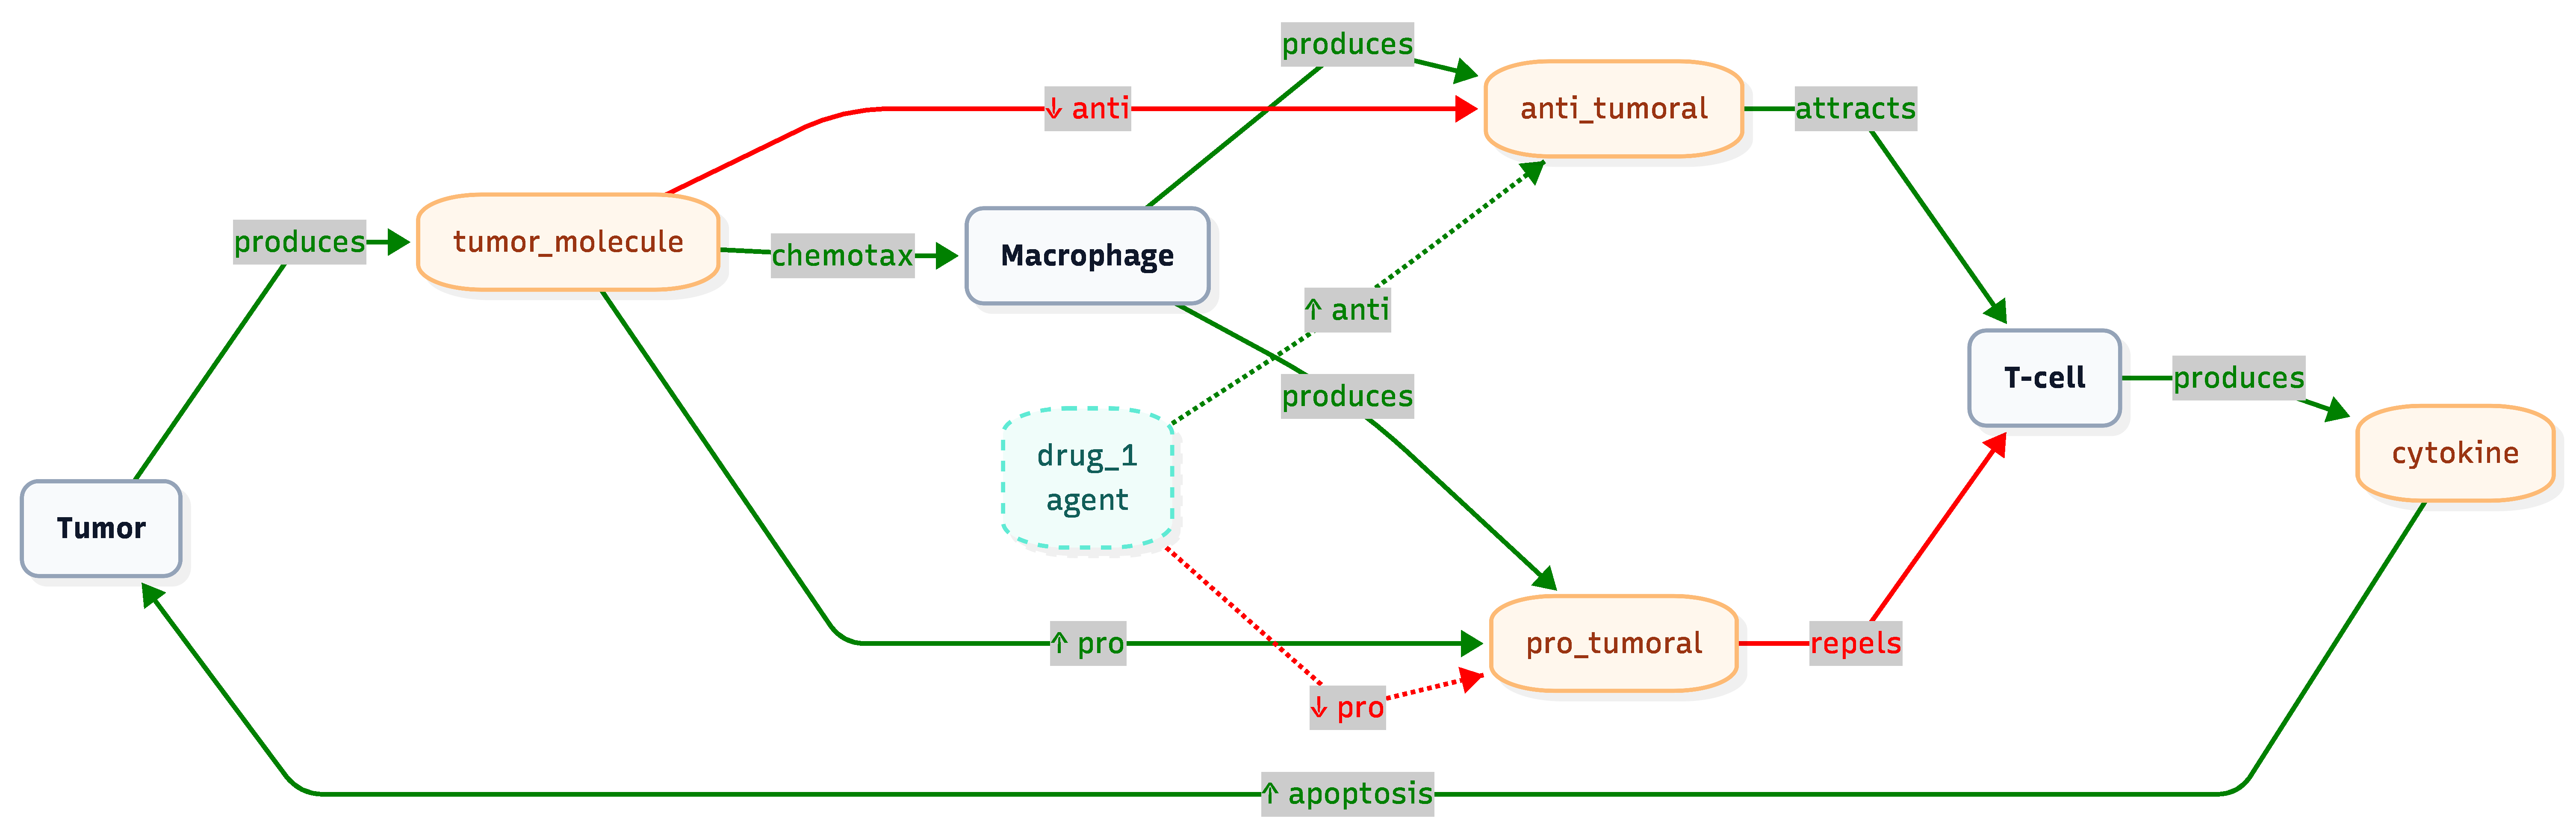
\includegraphics[width=1.1\linewidth]{img/fig_tme}
    \caption{Tumor Microenvironment (TME) signalling network. Green solid arrows denote production, activation, or attraction, while red solid arrows indicate suppression or repulsion. The dashed pathways represent the intervention of the agent-controlled drug (\texttt{drug\_1}), highlighting its role as an immune-modulator that repolarizes macrophages to indirectly drive T-cell mediated tumor apoptosis.}
    \label{fig:tme_network}
\end{figure}


\subsection{Implementation of an RL approach to control the TME}
\label{sec:rl}

Our overall objective is to achieve complete tumor eradication while minimizing
drug exposure. We describe the action space $A$, the reward $R$, and the
training and test distributions. The observation space $S$ is the component we
vary across experiments: in Section~\ref{sec:results} we compare six
observation modes to assess whether spatially explicit representations help
the agent learn and generalize on this toy model.

\paragraph{Action space.}
At each gym step the agent selects
$a_t = (\text{dose},\,x,\,y,\,r)\in[0,1]^4$,
where dose is the drug concentration applied, $(x,y)$ is the injection centre
(normalised domain coordinates), and $r$ is the injection radius (normalised
by the domain diagonal).

\paragraph{Reward.}
The reward is a normalised tumor-suppression signal minus a drug-cost penalty:
\begin{equation}
  r_t \;=\; w_{\text{cell}}\,
  \frac{c_{t-1} - c_t}{\,c_{t-1}(e^{\lambda\Delta t}-1)\,}
  \;-\; d_t,
  \label{eq:reward}
\end{equation}
where $c_t$ is the alive tumor-cell count at step $t$,
$\lambda$ is the intrinsic growth rate (from \texttt{PhysiCell\_settings.xml}),
$w_{\text{cell}}=0.3$, and $d_t$ is the normalised dose spent, keeping the learning signal clean: the
$d_t$ term already penalises drug use without conflating temporal dosing
strategy with total exposure.

\subsubsection*{Training and Test Distributions}
\label{sec:distributions}

To ensure the model learns robust policies rather than overfitting to specific spatial configurations, we evaluate on strictly held-out test distributions. While training initializations are sampled from a \emph{network-field} (detailed in Appendix~\ref{app:ic}), we test out-of-distribution (OOD) generalisation using two layouts never seen during training:
\begin{itemize}
    \item \textbf{Circular}: The tumour is placed within a domain-centred ellipse.
    \item \textbf{Rectangle}: Each cell type is placed uniformly in a narrow vertical strip.
\end{itemize}
Figure~\ref{fig:ic_distributions} illustrates representative examples of the training and OOD test distributions.

\subsection{State space $S$: observation spaces compared}
\label{sec:obs}

In a tumor microenvironment there are different cell types and different
molecules/chemical compounds (substrates). The simulator can expose several
kinds of data: some carry explicit spatial information, others are spaceless
summaries (e.g.\ a small vector of global statistics). Because \physigym{}
can build all of these from the same underlying simulation, we use the toy model
to study how the choice of observation space affects the dynamic treatment regime
that RL learns, comparing six modes on cumulative return and on generalization to
unseen spatial configurations.

We compare six observation modes spanning a spectrum from global scalars to
full spatial images.
Let $N_c=3$ (tumor, T-cell, macrophage) and $N_s=5$ substrates.

\subsubsection*{Scalar Observation Spaces}

\paragraph{S1 (Normalised Cell Count):}
Alive count per cell type, normalised to the initial population. Defined as $s_i = c_i(t)/c_{\text{init}} - 1$, where the initial count is $c_{\text{init}}=512$. 
\\ \textit{Space:} $\mathbb{R}^{N_c}$

\paragraph{S2 (Cell Count + Substrate Maxima):}
S1 augmented with the maximum spatial concentration for each substrate. For a given substrate $j$, this is defined as $s_j = \max_{\mathbf{x}} \mathrm{conc}_j(\mathbf{x},t)$. 
\\ \textit{Space:} $\mathbb{R}^{N_c + N_s}$

\paragraph{S3 (Per-Type Spatial Statistics):}
S1 combined with six spatial statistics per cell type: a presence flag, centroid coordinates $(x_\mu, y_\mu)$, spatial spread $(x_\sigma, y_\sigma)$, and distance to the domain centre. All values are normalised to the range $[0, 1]$. 
\\ \textit{Space:} $\mathbb{R}^{7N_c}$

\paragraph{S5 (Global Spatial Statistics):}
S3 extended with six global spatial statistics per substrate: mean, standard deviation, minimum, maximum, and the concentration-weighted centroid $(x_c, y_c)$. 
\\ \textit{Space:} $\mathbb{R}^{7N_c + 6N_s}$


\subsubsection*{Image-Based Observation Spaces}

\paragraph{I1 (Cell Types Only):}
One channel allocated per cell type. 
\\ \textit{Space:} $\mathbb{R}^{N_c \times 64 \times 64}$ (\texttt{uint8})

\paragraph{I2 (Cells + Substrates):}
I1 concatenated with all five substrate concentration maps. This richer observation provides direct spatial feedback on the macrophage polarisation state via the \texttt{pro\_tumoral}, \texttt{anti\_tumoral}, and \texttt{drug\_1} channels. 
\\ \textit{Space:} $\mathbb{R}^{(N_c + N_s) \times 64 \times 64}$ (\texttt{uint8})

\subsubsection*{Why substrate spatial maps close the feedback loop}

The indirect drug mechanism (Section~\ref{sec:model}) requires multi-step
credit assignment: the agent injects drug, macrophages polarise over several
steps, anti-tumoral gradients shift, T-cells migrate, cytokine rises, and
only then do tumor cells die.
Without substrate maps the agent observes only cell counts, and cannot
determine (i)~whether an injection reached macrophages, (ii)~whether
polarisation occurred, or (iii)~where T-cells will concentrate next.
The scalar max-concentration in S2 destroys spatial structure entirely.
Only I2's per-pixel substrate channels make the polarisation state and drug
distribution spatially legible at each step.

% ─────────────────────────────────────────────────────────────────────────────
\section{Results}
\label{sec:results}
% ─────────────────────────────────────────────────────────────────────────────

\subsection{Aggregated performance}

Table~\ref{tab:results} summarises final performance (seeds averaged).
Figures~\ref{fig:train_curves} and~\ref{fig:test_curves} show learning curves
vs.\ cumulative environment steps with mean $\pm$ std shading across seeds.

\begin{table}[h]
  \caption{Performance at end of training.
    Train$_\mu$/Test$_\mu$: mean smoothed return.
    Train$_\sigma$/Test$_\sigma$: std across seeds.}
  \label{tab:results}
  \centering\small
  \begin{tabular}{llccccccc}
    \toprule
    \textbf{ID} & \textbf{Mode} & \textbf{Dim} & \textbf{$n$} &
    \textbf{Train$_\mu$} & \textbf{Train$_\sigma$} &
    \textbf{Test$_\mu$}  & \textbf{Test$_\sigma$} \\
    \midrule
    I2 & img + substrates   & $8{\times}64^2$ & 5 & \textbf{+77.2} & 8.5  & \textbf{+56.5} & 10.3 \\
    I1 & img cells only     & $3{\times}64^2$ & 4 & +50.3          & 11.3 & +20.8          & 18.2 \\
    \midrule
    S3 & spatial cells      & 21              & 3 & +51.2          & 25.8 & +12.4          & 34.6 \\
    S5 & spatial cells+subs & 39              & 2 & +3.2           & 7.3  & +0.5           & 0.5  \\
    S2 & scalar cells+subs  & 8               & 4 & $-16.8$        & 38.3 & +12.3          & 27.0 \\
    S1 & scalar cells       & 3               & 4 & +5.9           & 22.0 & +17.6          & 22.5 \\
    \bottomrule
  \end{tabular}
\end{table}

\begin{figure}[h]
  \centering
  
\includegraphics[width=\linewidth]{img/train_return_mean50.pdf}
  \caption{Training return (EWMA-50, mean $\pm 1\sigma$ across seeds) vs.\
    cumulative environment steps ($\times 10^5$).
    I2 (red) separates from all other modes after $\approx\!0.5\!\times\!10^5$
    steps and widens the gap throughout training.
    Scalar modes plateau below $+35$ and exhibit high inter-seed variance
    (shaded bands).}
  \label{fig:train_curves}
\end{figure}

\begin{figure}[h]
  \centering
  
\includegraphics[width=\linewidth]{img/return_std.pdf}
  \caption{Standard deviation of return across seeds vs.\ environment steps:
    training (left) and test (right).
    Image modes (I1, I2) maintain consistently lower std than scalar modes
    throughout training.
    I2's train std (${\approx}8.5$) is 3--4$\times$ lower than S2's (${\approx}38.3$),
    confirming that spatial substrate representations produce more robust
    learning dynamics across random initialisations.}
  \label{fig:std_curves}
\end{figure}

\begin{figure}[h]
  \centering
  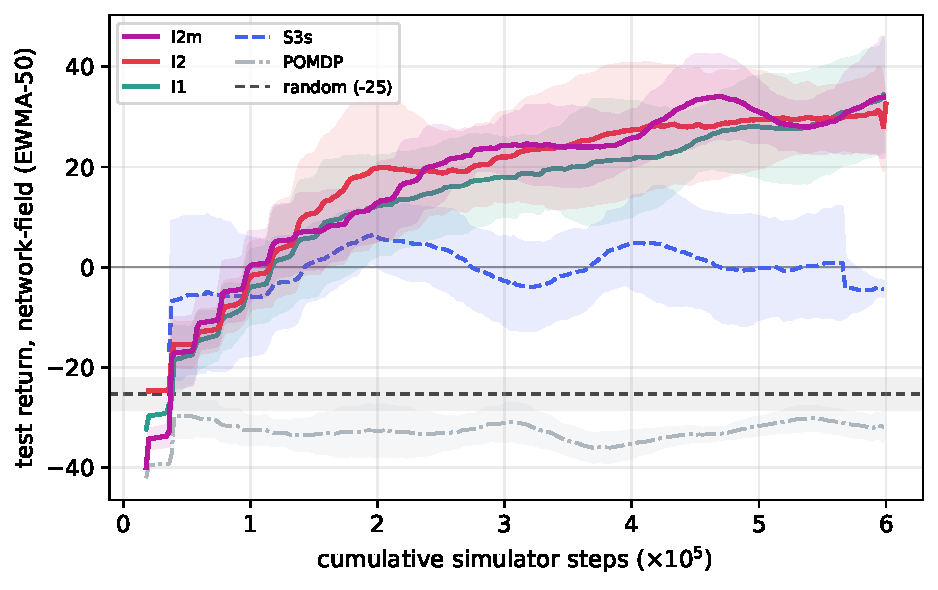
\includegraphics[width=\linewidth]{img/test_return_mean50.pdf}
  \caption{Test return (mean $\pm 1\sigma$ across seeds, EWMA-50) vs.\
    cumulative environment steps.
    Test episodes alternate between circular and rectangle held-out layouts.
    I2 consistently climbs throughout training; I1 and scalar modes show
    little improvement and high variance, confirming that substrate spatial
    information is required for generalisation to OOD layouts.}
  \label{fig:test_curves}
\end{figure}

\subsection{Key findings}

\paragraph{Substrate channels are decisive.}
Adding substrate maps to the cell-only image (I1$\to$I2) raises training
return by $+27$ and test return by $+36$ points  the largest single
improvement in the comparison.
Adding substrate \emph{scalars} (S1$\to$S2) gives $-22$ points on training
return and raises seed variance to $\sigma=38.3$, confirming that spatially
aggregated substrate values are not only insufficient but harmful.

\paragraph{More scalar features does not help.}
Scalar complexity increases S1(3)$\to$S2(8)$\to$S3(21)$\to$S5(39), but
train mean follows $+5.9\to-16.8\to+51.2\to+3.2$.
S3's centroid statistics help; adding substrate spatial statistics (S5) hurts,
likely because the 39-dim space is harder to optimise in 500k steps.

\paragraph{Seed robustness.}
Image modes show 3--4$\times$ lower seed variance than scalar modes
(Table~\ref{tab:results}, Figure~\ref{fig:train_curves} right).
I2's train std is $8.5$ vs.\ S2's $38.3$.
The CNN inductive bias (spatial locality, translation equivariance) aligns
with the TME's physical structure and consistently guides optimisation
regardless of random initialisation.

\subsection{Generalisation to held-out layouts}

\begin{table}[h]
  \caption{Test return by held-out layout (seeds averaged).}
  \label{tab:layouts}
  \centering\small
  \begin{tabular}{lrrr}
    \toprule
    \textbf{Mode} & \textbf{Test avg} & \textbf{Rectangle} & \textbf{Circular} \\
    \midrule
    I2 & \textbf{+56.5} & +44.5 & \textbf{+97.9} \\
    I1 & +20.8          & $-0.6$ & +5.0 \\
    S3 & +12.4          & \textbf{+112.7} & +16.3 \\
    S5 & +0.5           & +85.1 & $-37.6$ \\
    S2 & +12.3          & +40.2 & $-47.7$ \\
    S1 & +17.6          & $-7.7$ & $-20.5$ \\
    \bottomrule
  \end{tabular}
\end{table}

I2 achieves the highest \emph{average} test return and the highest circular
return ($+97.9$).
I1 fails on both OOD layouts (near zero or negative), confirming that
cell-image policies overfit to the training network-field geometry without
substrate feedback.
The S3 rectangle outlier is a single seed; its circular return is $+16.3$,
illustrating the inconsistency of scalar-mode generalisation.

Appendix~\ref{app:episodes} shows two matched episodes examples (run\_000143 and
run\_000147) comparing I2, I1, and S3 step-by-step, illustrating the
two failure modes that summarise the whole comparison: I1 under-medicates
because without substrate channels it cannot assess whether injections
reached macrophages; S3 achieves early suppression but cannot finish
because it lacks the substrate spatial feedback needed to target the
final push to eradication.

% ─────────────────────────────────────────────────────────────────────────────
\section{Discussion}
% ─────────────────────────────────────────────────────────────────────────────

The central outcome of this work is \physigym{} itself: a framework that lets
RL agents control a full agent-based TME through a standardised interface,
without recompilation, and with arbitrary observation and action spaces. The
toy-model case study shows the framework end-to-end  an agent learns a spatial
drug-delivery policy that steers the microenvironment toward an anti-tumoral
state and, in the best episodes, eradicates the tumor.

The toy model also produces a clear result on observation spaces. Spatially
explicit (image) observations consistently outperform global scalar summaries,
and substrate spatial maps are the most informative of all: the CNN in I2 can
compute cross-channel co-localisation statistics (e.g.\ whether \texttt{drug\_1}
and macrophages overlap at the same location) that would require explicit
engineered features in any scalar representation, while the scalar
max-concentration in S2 discards spatial structure entirely. The same ordering
holds for generalization to held-out layouts: I2 transfers because substrate
gradients are spatially informative regardless of initial geometry, whereas
scalar modes encoding absolute centroid positions tend to overfit to the
training distribution.

We emphasise that this is an application-level observation on a deliberately
simplified model, not a universal claim about biological control. In more
complex or realistic models  or with different reward designs, action spaces,
or RL algorithms  the relative value of cell versus substrate, and scalar
versus image, may differ. \physigym{} is precisely the tool that makes such
questions answerable in a reproducible way.

\paragraph{Limitations.}
The toy model is intentionally small (64\,$\mu$m, 2D) and cheap to simulate.
Scaling to 3D or larger domains will increase the cost of image observations.
All experiments use a single RL algorithm (SAC); alternative algorithms or
model-based methods may interact differently with observation spaces.
Complex biological models and/or 3D models are left to future work.

% ─────────────────────────────────────────────────────────────────────────────
\section{Conclusion}
% ─────────────────────────────────────────────────────────────────────────────

We presented \physigym{}, an open-source framework that bridges the
\physicell{} ABM with Gymnasium RL, enabling direct policy learning in
spatially explicit biological simulations.
Using a TME model with an indirect drug mechanism, we showed that full
spatial substrate images are the critical state representation: they raise
training return by $+71$ points and test return by $+39$ points over pure
scalar baselines.
The mechanism is causal  substrate maps close the feedback loop between drug
injection and macrophage repolarisation that is invisible to all scalar modes.
\physigym{} provides the infrastructure to study such questions in a
principled, reproducible manner, and we anticipate it will serve as a
testbed for both computational biology and RL communities.

% ─────────────────────────────────────────────────────────────────────────────
\begin{ack}
A.B., V.P., and E.R.\ acknowledge funding from Region Occitanie and INSERM,
Projet Emergence REACT.
E.B.\ received support from a Chateaubriand Fellowship of the Office for
Science \& Technology of the Embassy of France in the United States.
This study was partially supported through grant EUR CARe N°ANR-18-EURE-0003
and an Eiffel Excellence doctoral fellowship to M.H.
This research was also supported in part by Lilly Endowment, Inc., through its
support for the Indiana University Pervasive Technology Institute.
No competing interests are declared.
\end{ack}

% ─────────────────────────────────────────────────────────────────────────────
\bibliographystyle{abbrvnat}
\bibliography{reference}

% ─────────────────────────────────────────────────────────────────────────────
\appendix

\section{Generation of Initial Conditions}
\label{app:ic}
White Gaussian noise $\eta(\mathbf{x})\sim\mathcal{N}(0,1)$ is convolved
with a Gaussian kernel $G_\sigma$ ($\sigma=\ell_c/\sqrt{2}$,
$\ell_c=45$\,µm) to produce a correlated field $F$.
An additional local noise component $\tilde\xi$ filtered at width
$\ell_c/3$ is added with small weight $\alpha$ to introduce local
heterogeneity.
The field is normalised to $[0,1]$ and cells are sampled from positions
with $\hat{F}>0.55$, with probability proportional to $\hat{F}$.

For the circular test layout, tumor cells are placed in a random ellipse
(semi-axes $r_1 \in [0.1,0.4]$, $r_2 \in [0.1,0.4]$ of the half-domain)
centred on the domain, and immune cells in two flanking ellipses at 20\%
and 80\% of the $x$-axis (shuffled between T-cells and macrophages).
For the rectangle layout, each cell type is placed uniformly in a vertical
strip of width 10\% of the $x$-axis, with non-overlapping strip positions
sampled from $[0.1,0.2]$, $[0.3,0.5]$, $[0.6,0.8]$ (shuffled across types).

\begin{figure}[htbp]
    \centering
    % Adjust the width as needed (e.g., 0.8\linewidth, or a specific size like 8cm)
    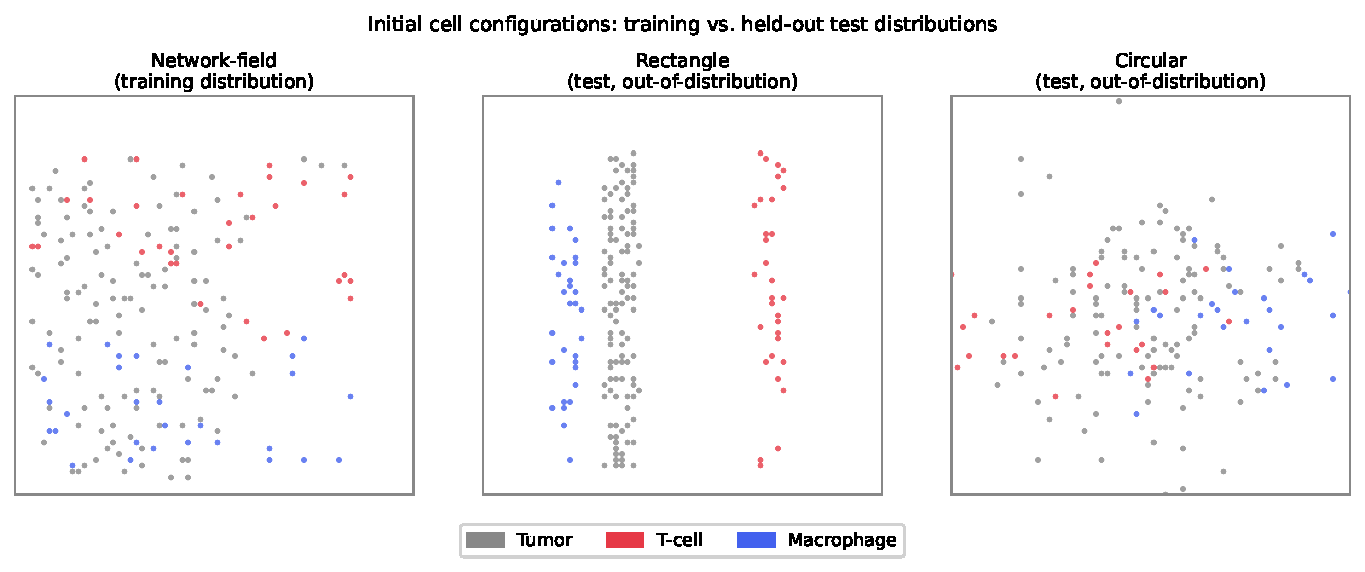
\includegraphics[width=\linewidth]{img/ic_distributions}
    \caption{Representative examples of the training (network-field) and out-of-distribution (circular and rectangle) spatial layouts.}
    \label{fig:ic_distributions}
\end{figure}



\section{Training algorithm and setup}
\label{sec:training}

To address our control objective  maximizing cancer-cell eradication while
minimizing drug administration  we employ Soft Actor-Critic
(SAC)~\citep{haarnoja2018soft}, a state-of-the-art RL algorithm for continuous
control. SAC is well suited to our setting due to its high sample efficiency,
and as a deep RL method it accommodates different observation types, such as
image-based representations, through Convolutional Neural Networks
(CNNs)~\citep{o2015introduction}. A key challenge is the computational cost of
the simulator; to alleviate this bottleneck we adopt an asynchronous parallel
training framework~\citep{mnih2016asynchronous, liu2025asynchronous}.
A GPU-resident learner updates policy and value networks asynchronously while
9 CPU-resident environment processes generate experience in parallel.

\subsection{Asynchronous SAC}
\label{app:async_sac}

\begin{algorithm}[H]
\caption{Asynchronous SAC with Parallel Environments~\citep{liu2025asynchronous}}
\label{alg:async_sac}
\begin{algorithmic}[1]
\Require Config $d_\text{arg}$, buffer size $|\mathcal{B}|$, LRs, $\gamma$, $\tau$
\State Init shared queues \texttt{actor\_queue}, \texttt{sample\_queue};
       stop signal \texttt{stop\_event}
\State \textbf{Actor Process (CPU):} init $N_\text{env}=9$ envs, local $\pi_{\theta_a}$
\While{not \texttt{stop\_event}}
  \State Receive $\theta$ from \texttt{actor\_queue} if available
  \State Act: random if $t\!<\!T_\text{start}$, else $\pi_{\theta_a}$
  \State Step envs; push $(s,a,r,s',d)$ to \texttt{sample\_queue}
\EndWhile
\State \textbf{Learner Process (GPU):} init $\pi_\theta$, $Q_{\phi_{1,2}}$, targets, $\mathcal{D}$
\While{total samples $< T$}
  \State Drain \texttt{sample\_queue} into $\mathcal{D}$
  \For{$N_\text{loops}$ gradient steps}
    \State Sample minibatch; compute SAC target $y$; update $Q$, $\pi$, $\alpha$;
           soft-update targets
  \EndFor
  \State Push updated $\theta$ to \texttt{actor\_queue}
\EndWhile
\end{algorithmic}
\end{algorithm}

\subsection{Neural Architecture}

\textbf{Scalar modes} utilize a Multi-Layer Perceptron (MLP):
\[
\mathrm{FC}(256) \xrightarrow{\text{Mish}} \mathrm{FC}(256)
\]

\textbf{Image modes} utilize an IMPALA-style CNN~\citep{espeholt2018impala}. The feature extraction and projection pipeline is defined as:
\begin{align*}
    &\mathrm{Conv}(n_c \to 32,\, k{=}8{\times}8,\, s{=}4) \xrightarrow{\text{Mish}} \\
    &\mathrm{Conv}(32 \to 64,\, k{=}4{\times}4,\, s{=}2) \xrightarrow{\text{Mish}} \\
    &\mathrm{Conv}(64 \to 64,\, k{=}3{\times}3,\, s{=}1) \xrightarrow{\text{Mish}} \mathrm{Flatten} \xrightarrow{} \mathrm{FC}(256) \xrightarrow{} \mathrm{FC}(256)
\end{align*}

\subsection{Hyperparameters}
\label{app:hyperparams}

\begin{table}[h]
  \centering\small
  \caption{SAC hyperparameters (TME v2 experiments).}
  \label{tab:hyperparams}
  \begin{tabular}{lll}
    \toprule
    \textbf{Parameter} & \textbf{Symbol} & \textbf{Value} \\
    \midrule
    Total training steps & $T$              & $5\!\times\!10^5$ \\
    Replay buffer size   & $|\mathcal{B}|$  & $3\!\times\!10^5$ \\
    Batch size           & $B$              & 576 \\
    Warm-up steps        & $T_\text{start}$ & 5{,}000 \\
    Policy / critic LR   & $\eta_\pi,\eta_Q$& $3\!\times\!10^{-4}$ \\
    Discount factor      & $\gamma$         & 0.99 \\
    Target smoothing     & $\tau$           & 0.005 \\
    Entropy autotuning   & --               & enabled \\
    Parallel envs        & $N_\text{env}$   & 9 \\
    Update loops / step  & $N_\text{loops}$ & 3 \\
    Test frequency       & --               & every 4 episodes \\
    \bottomrule
  \end{tabular}
\end{table}



\section{Example Episode Comparisons}
\label{app:episodes}

Figures~\ref{fig:episode} and~\ref{fig:episode2} show two matched test
episodes comparing I2 (\Itwo{}), I1 (\Ione{}), and S3
(\Sthree{}) step by step.  All three agents start from identical initial
conditions; the only difference is the observation mode.

\begin{figure}[h]
  \centering
  
\includegraphics[width=\linewidth]{img/fig_episode_comparison.pdf}
  \caption{\textbf{run\_000143, seed~64  near-eradication episode.}
    Cumulative return (top), cumulative drug used (middle), per-step dose (bottom).
    I2 reaches near-eradication (4 tumor cells remaining, $+175$ return, 35.4 total dose).
    S3 achieves partial control (14 cells, $+106$ return, 31.1 total dose).
    I1 fails entirely (112 cells, $-7.4$ return, 12.2 total dose).
    Despite comparable total drug between I2 and S3, only I2 eradicates
    the tumor: substrate maps allow precise placement that converts dose
    into effective macrophage repolarisation.
    I1 under-medicates throughout  without substrate feedback the agent
    cannot evaluate whether injections were effective.}
  \label{fig:episode}
\end{figure}

\begin{figure}[h]
  \centering
  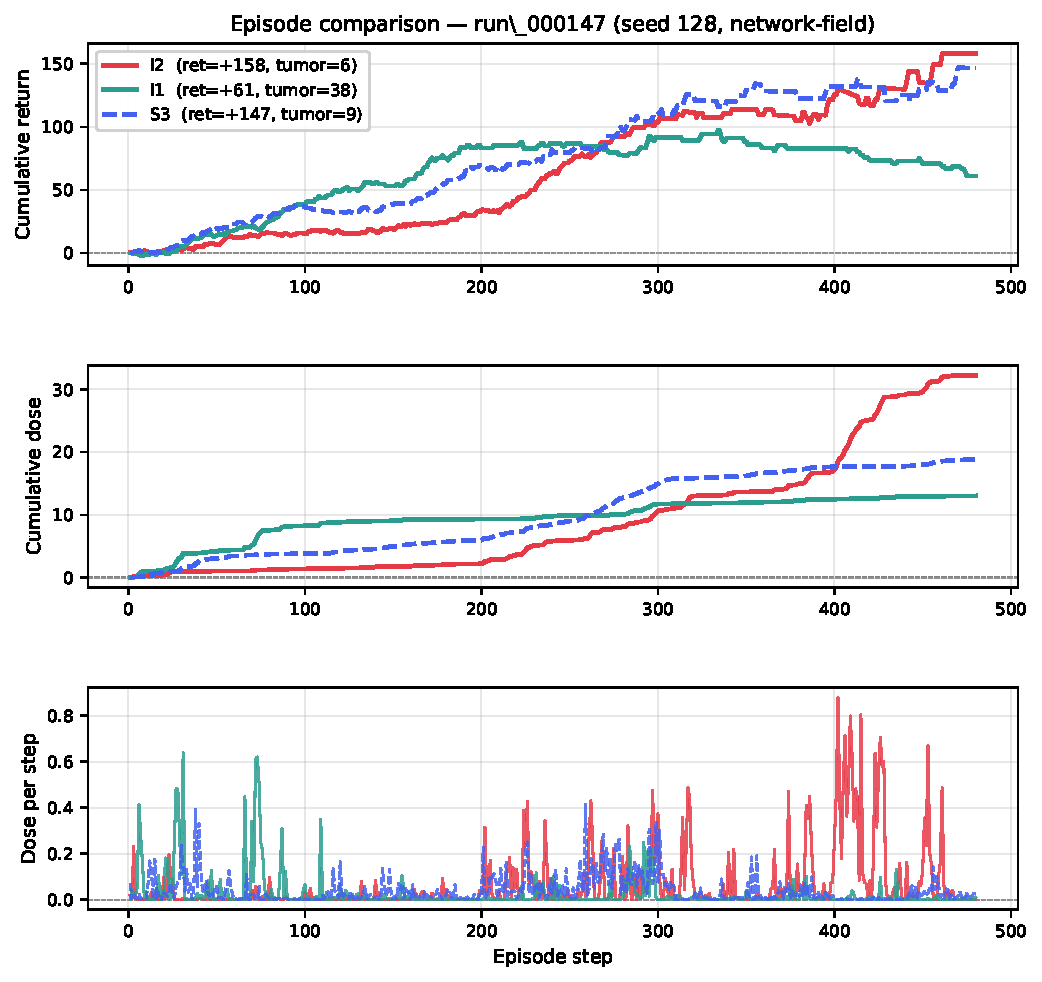
\includegraphics[width=\linewidth]{img/fig_episode_comparison_2.pdf}
  \caption{\textbf{run\_000147, seed~128  harder episode with tumor rebound.}
    No agent reaches eradication.
    I2: $+158$ return (6 tumor cells, 32.2 total dose).
    S3: $+147$ return (9 cells, 18.9 total dose).
    I1: $+61$ return (38 cells, 13.0 total dose).
    All three agents build positive return through step~$\approx$330, then
    the tumor rebounds; I2 best contains the rebound.
    The two failure modes identified in run\_000143 persist: I1 under-medicates
    (13.0 vs.\ 32.2 for I2), and S3 cannot sustain control without substrate
    spatial feedback to track the evolving immunosuppressive gradient.
    Contrasting the two episodes: the advantage of I2 is largest when
    eradication is reachable; when the tumor is more resilient all modes
    struggle, but I2 still maintains the best outcome.}
  \label{fig:episode2}
\end{figure}



\end{document}
